\section{ProtoDUNE-ND detector physics studies}
\label{sec:detector-physics-studies}
Basic detector stability checks will be checked with a period of detector operation in Bern before moving the module to Fermilab. These tests would include extraction and re-insertion tests of individual modules into the LAr bath, and checks that the LAr purity is sufficient. However, local tests can only be performed using cosmic muons, which have limited utility beyond basic detector stability checks. In this section, we identify a number of key detector physics questions which could be answered by the ProtoDUNE-ND test, and would help inform the final design of the full ArgonCube ND component for DUNE, and aid in developing reconstruction algorithms suitable for neutrino interactions.

In order to check the feasibility of these studies, two different simulations were used. Firstly, high statistics GENIE Monte Carlo samples were produced, in order to compare basic properties of neutrino interactions expected in the LBNF and NuMI ME beamlines. Secondly, GENIE events were used to seed a basic GEANT4 simulation, using the ArgonBox software, in order to get a basic understanding of event shape and containment. In the latter simulation, events were simulated in an infinite box of LAr, and were then distributed randomly inside a volume with the correct spatial dimensions as the 2x2 demonstrator module. Although the 2x2 geometry was not included in the simulation, this gives an acceptable estimate of the expected event rates for the studies described below. \todo{Patrick/Chris to expand this clumsy description of ArgonBox. Is there a reference I should use?}. Examples of the ArgonBox simulation with the basic 2x2 geometry superimposed can be seen in Figure~\ref{fig:argonbox_event_display} for a number of different neutrino energies.

\begin{figure}[htb]
  \centering
  \subfloat[$E_{\nu}$ = 2.60 GeV] {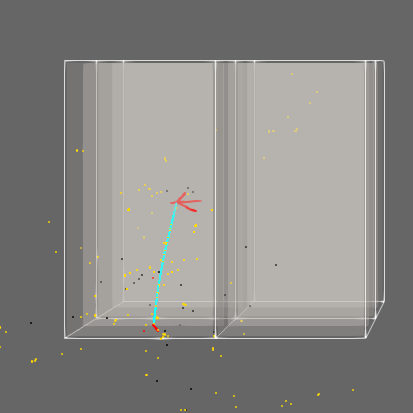
\includegraphics[width=0.45\textwidth]{{plots/EventDisplays/2.60GeV_square_crop}.png}}\hspace{25pt}
  \subfloat[$E_{\nu}$ = 3.36 GeV] {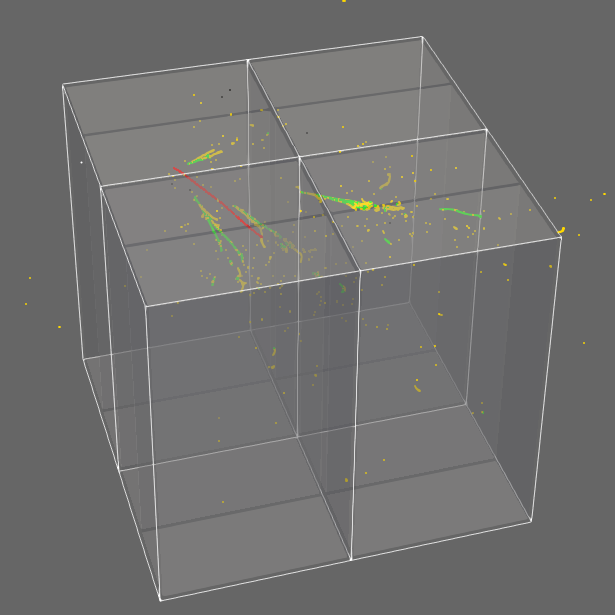
\includegraphics[width=0.45\textwidth]{{plots/EventDisplays/3.36GeV_square_crop}.png}}\\
  \subfloat[$E_{\nu}$ = 4.83 GeV] {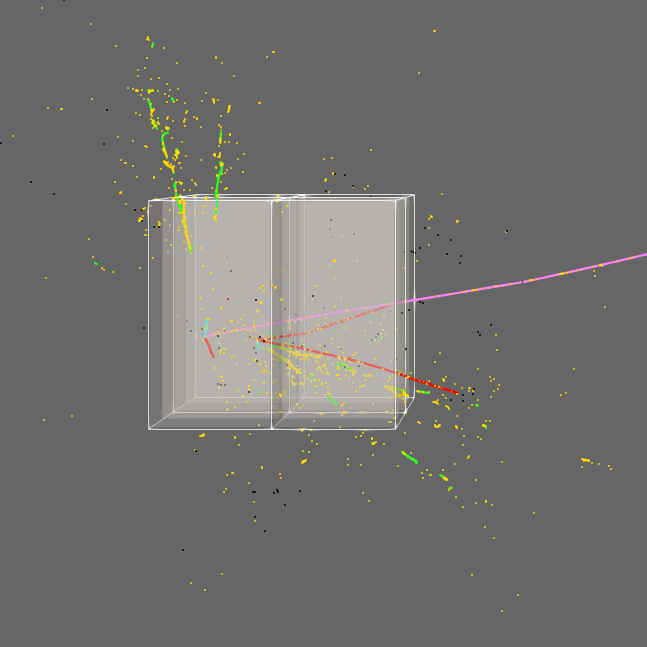
\includegraphics[width=0.45\textwidth]{{plots/EventDisplays/4.83GeV_square_crop}.png}}\hspace{25pt}
  \subfloat[$E_{\nu}$ = 9.37 GeV] {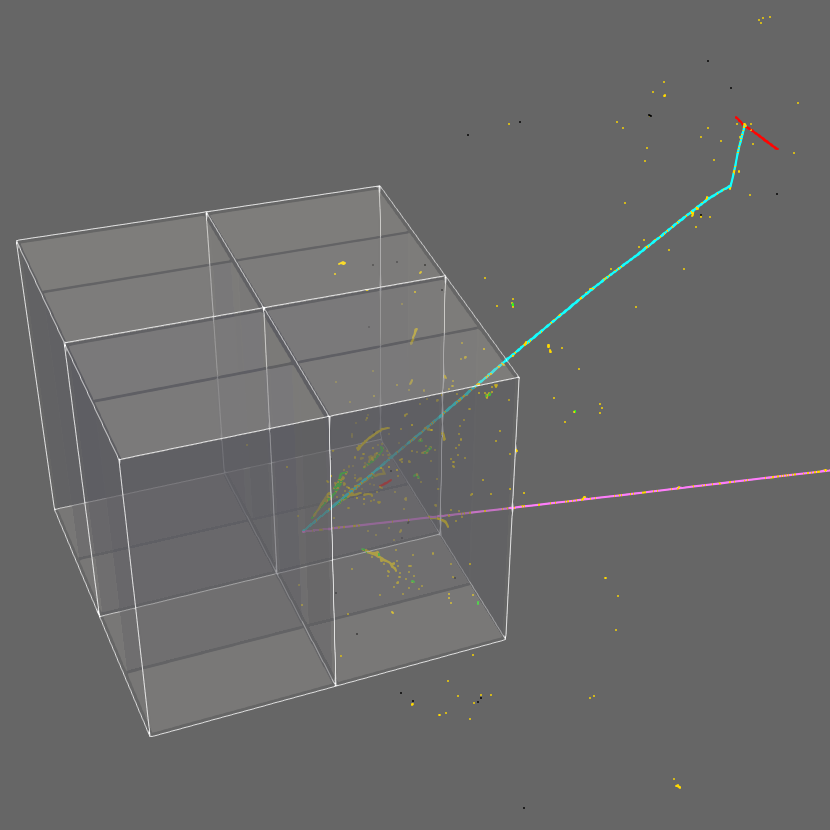
\includegraphics[width=0.45\textwidth]{{plots/EventDisplays/9.37GeV_square_crop}.png}}
  \caption{Example $\nu_{\mu}$--argon ArgonBox simulated events for a number for different incident neutrino energies, where the energy deposits in a bulk volume of LAr are color-coded according to the particle type: $\pi^{\pm}$ --- blue; $\mu^{\pm}$ --- purple; $e^{+}$ --- green; $e^{-}$ --- yellow; proton --- red; recoiling nuclei --- black. The event vertices are randomly placed within the active volume of the 2x2 demonstrator module, the geometry for which is superimposed on these images, but which is not simulated by ArgonBox.}
  \label{fig:argonbox_event_display}
\end{figure}

The example event displays shown in Figure~\ref{fig:argonbox_event_display} give a basic idea of how NuMI ME energy events (in FHC) would look in the ArgonCube 2x2 Demonstrator module. Although many of the tracks and showers are not contained, some fraction are, which is discussed in more detail for the detector physics studies described below. It also suggests that some fraction of the events seen in the 2x2 would be fully contained in the active volume, or fully contained except for the outgoing muon, which may open the way for some interesting physics studies beyond the detector physics described in this document. However, any possible utility in this direction would be severly limited without a downstream tracker to contain higher momentum hadronic components, and to tag the muon. This makes the case for adding an additional ProtoDUNE-ND test module for a HPTPC downstream tracker even stronger, or if that proves not to be possible on the timescale of this test, utilizing the existing MINERvA or MINOS-ND detectors in the experimental hall.

\begin{figure}[htb]
  \centering
  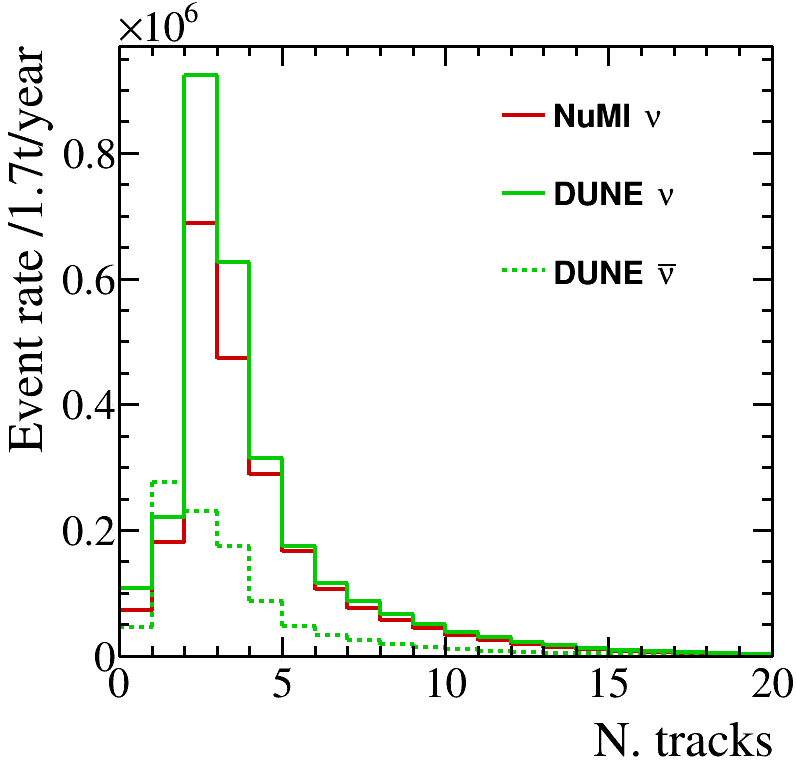
\includegraphics[width=0.5\textwidth]{plots/2x2_ntracks_all.png}
  \caption{The expected yearly rates of minimum and highly ionizing particles expected in the 2x2 module's 1.7t LAr volume for the NuMI ME and LBNF fluxes, produced using GENIE v2.12.8 with the ``ValenciaQEBergerSehgalCOHRES'' configuration~\cite{genie}.}
  \label{fig:track_multiplicity}
\end{figure}
In order to be a relevant test for the full ArgonCube near detector, which will be in the LBNF beamline, it is useful to verify that the basic properties of the events are similar, despite the NuMI ME beam being somewhat higher energy than the planned LBNF beam (as shown in Figure~\ref{fig:beam_options}). Figure~\ref{fig:track_multiplicity} shows the expected multiplicity of minimum or highly ionizing tracks at the vertex for both the LBNF and NuMI ME beams, in neutrino and antineutrino mode, produced with the GENIE generator. The track multiplicities are similar, which indicates that the scale of the reconstruction problem is similar, and the proposed ProtoDUNE-ND test will be a useful benchmark for developing the ArgonCube reconstruction software.

\begin{figure}[htb]
  \centering
  \subfloat[$\mu^{\pm}$] {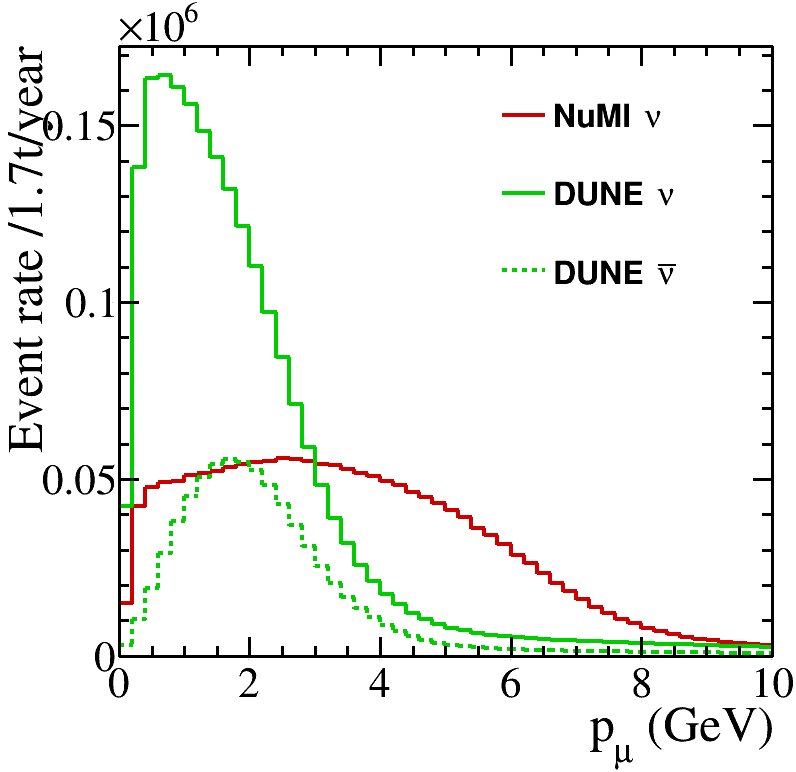
\includegraphics[width=0.5\textwidth]{plots/2x2_muon_mom_all.png}}
  \subfloat[Protons]    {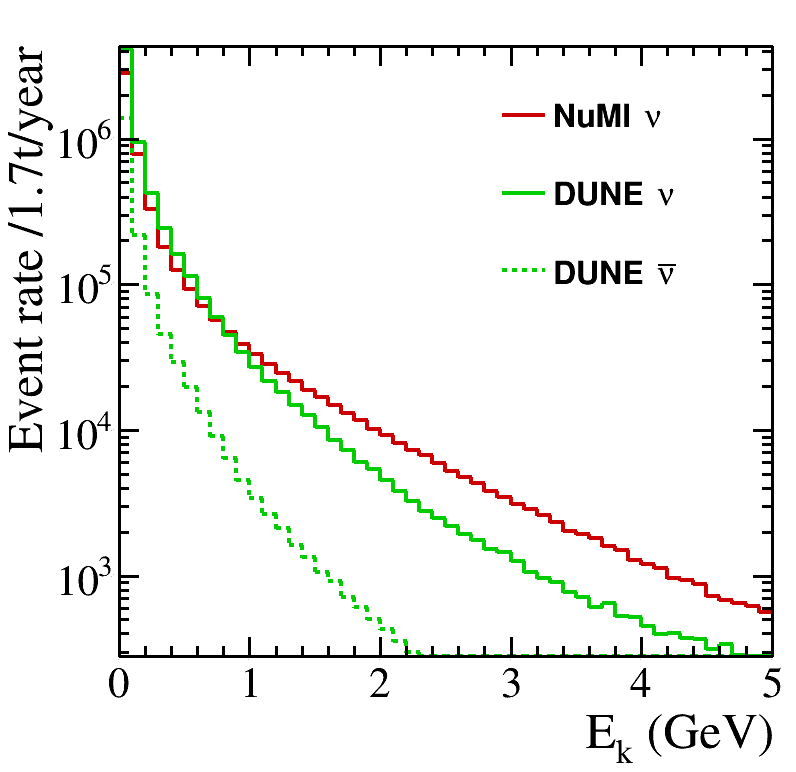
\includegraphics[width=0.5\textwidth]{plots/2x2_proton_Ek_all.png}}\\
  \subfloat[$\pi^{+}$]    {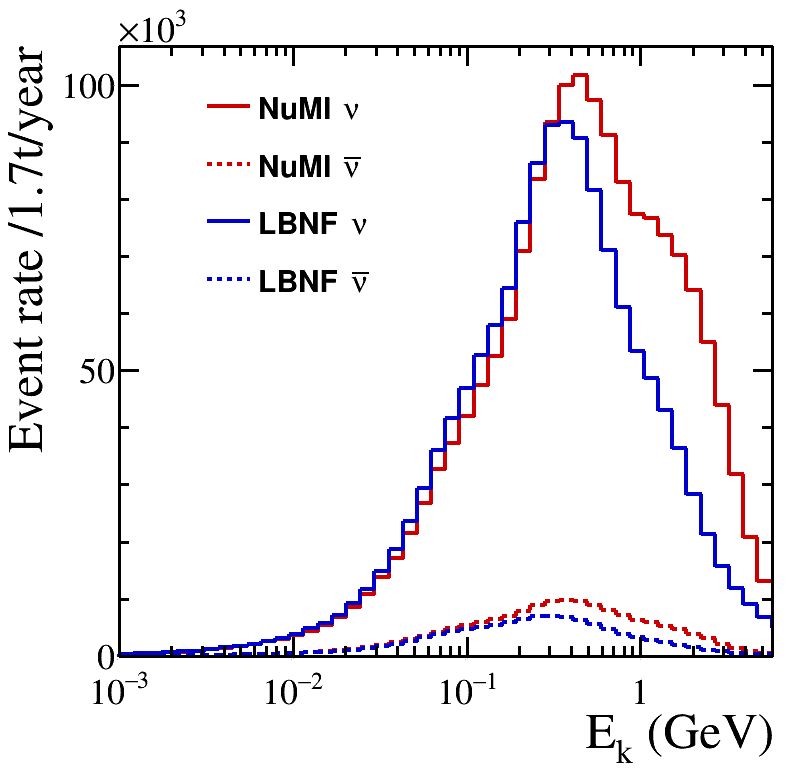
\includegraphics[width=0.5\textwidth]{plots/2x2_piplus_Ek_all.png}}
  \subfloat[$\pi^{-}$]    {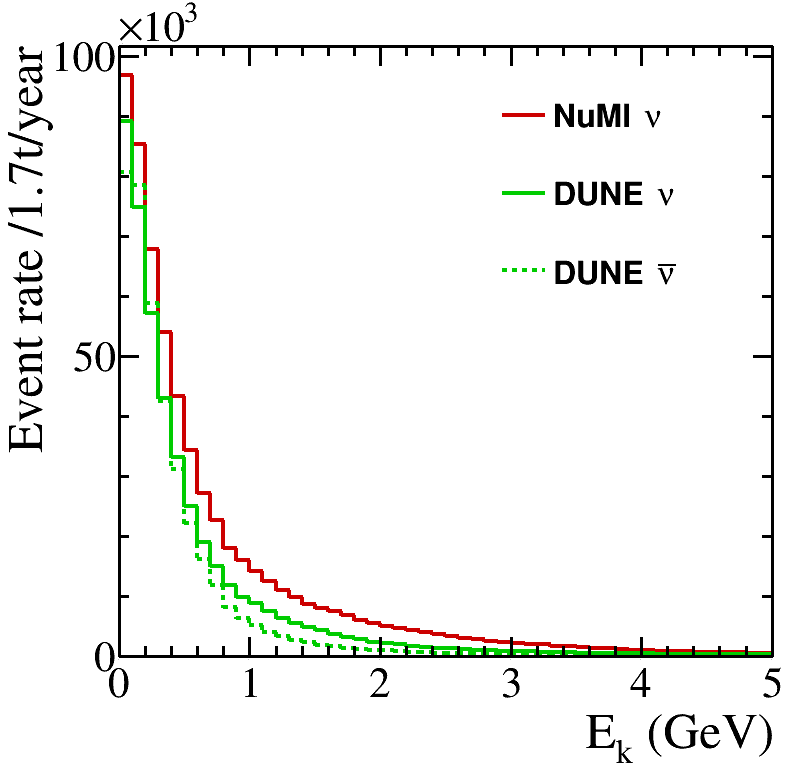
\includegraphics[width=0.5\textwidth]{plots/2x2_piminus_Ek_all.png}}  
  \caption{The expected yearly rates of various particles produced at the vertex, as a function of their kinetic energy, expected in the 2x2 module's 1.7t LAr volume for the NuMI ME and LBNF fluxes, produced using GENIE v2.12.8 with the ``ValenciaQEBergerSehgalCOHRES'' configuration~\cite{genie}. Note that every relevant particle from each event is included. \todo{Get the muon kinetic energy!}}
  \label{fig:kinetic_energies}
\end{figure}
In Figure~\ref{fig:kinetic_energies}, the kinetic energies of various particles coming from the initial neutrino--argon vertex are compared for the LBNF and NuMI ME beams. As expected, the energy distributions of all of the particles are slightly broader for the NuMI ME flux, but there are significant numbers of events with particle kinematics across the broad range of energies expected for the LBNF beams.

In the full ArgonCube detector and the more intense LBNF beamline, pile-up will be an additional challenge. \todo{Patrick to add a comment on pile-up at NuMI}. Additionally, the relatively small size of the 2x2 Demonstrator module means that relatively fewer of the tracks will be contained, making particle identification (PID) studies challenging, except for the cases listed below. Although other detectors are not included in the ArgonBox simulation, the lack of containment and PID capabilities mean that including another subdetector in the ProtoDUNE-ND setup is essential for any ancilliary physics measurements to be made.

\FloatBarrier
\subsection{Combining light and charge signals}
An important challenge is to develop automated event reconstruction software with the ArgonCube detector. The pixel readout removes the ambiguities present for projective wire readout TPCs, but the reconstruction software for the latter has benefitted from several years of development for the MicroBooNE~\addcite and ICARUS experiments~\addcite. Although strides forward for pixel readout TPCs have been made forward in the PixLAr experiment~\addcite (where pixel planes were introduced to the LArIAT experiment~\addcite), the reconstruction problem for charge particle scattering in a small TPC is much simpler than for the ProtoDUNE-ND or DUNE ND environments. Additionally, the recomstructed track position along the drift direction, and the suppression of cosmic backgrounds within the beam window, will be performed using information from the ArcLight light collection system. Checking that the light and charge signals can be combined in the full-size ArgonCube modules, in a comparably noisy environment to the DUNE ND, is an essential test of the ArgonCube design.

\subsection{Neutron identification}

\todo{Patrick's note. Quantitative test of how well we can combine light and charge signals.}
\begin{figure}[htb]
  \centering
  \subfloat[Neutron multiplicity]   {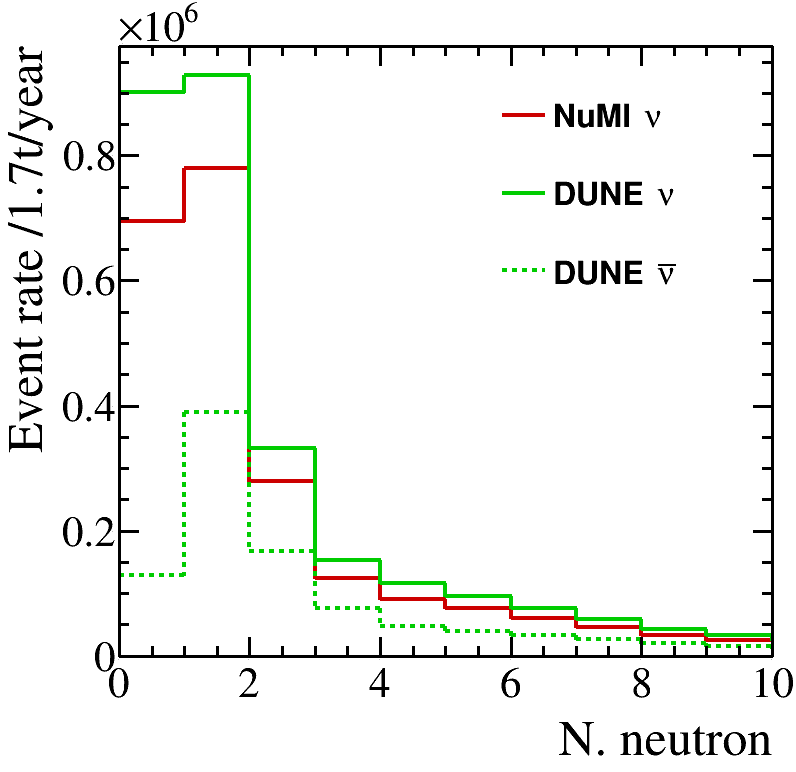
\includegraphics[width=0.5\textwidth]{plots/2x2_nneutron_all.png}}
  \subfloat[Neutron kinetic energy] {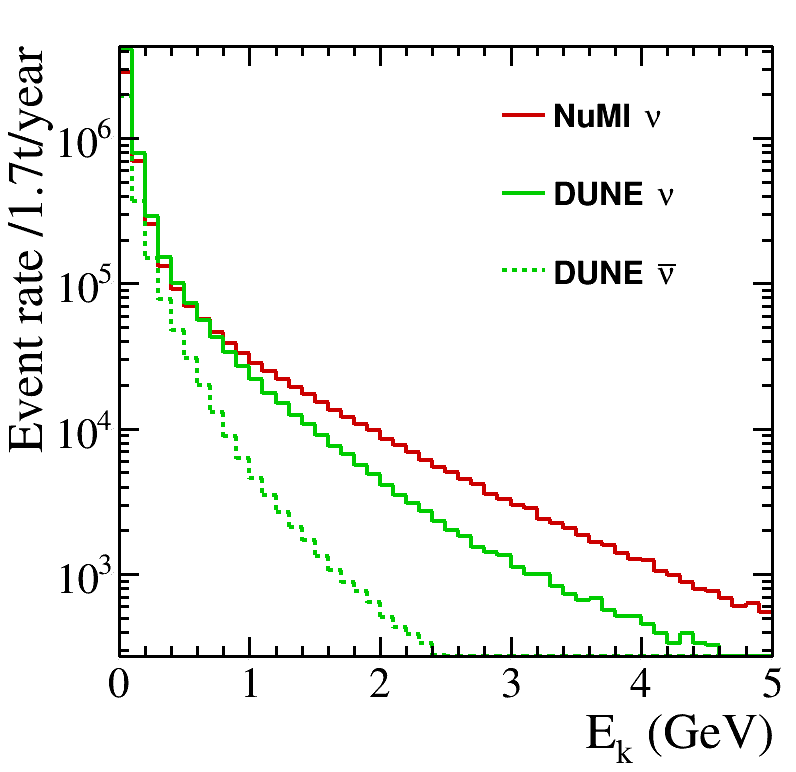
\includegraphics[width=0.5\textwidth]{plots/2x2_neutron_Ek_all.png}}  
  \caption{The expected yearly rates of $\pi^{0}$'s produced at the vertex, as a function of event multiplicity and their kinetic energy, expected in the 2x2 module's 1.7t LAr volume for the NuMI ME and LBNF fluxes, produced using GENIE v2.12.8 with the ``ValenciaQEBergerSehgalCOHRES'' configuration~\cite{genie}. Note that every $\pi^{0}$ from each event is included.}
  \label{fig:pi0_kinematics}
\end{figure}

\todo{Get the source for Patrick's neutron document. Steal some...}

\FloatBarrier
\subsection{Reconstruction in a modular environment}
\todo{James, please clarify and expand this!}
The module walls of the ArgonCube design produce gaps in particle tracks traversing multiple modules similar to dead wires in classic LArTPC readouts. Algorithms to join such segmented tracks already exist~\cite{pandora}, but have not been adapted to the ArgonCube design. Simple track matching efficiencies across modules can be calculated using cosmics, which will be an essential first step. However, for events with many tracks produced at the vertex (see Figure~\ref{fig:track_multiplicity}), a detailed study of the reconstruction performance given the module walls will need to be carried out. ProtoDUNE-ND provides an opportunity to do so, and to check that the reconstruction behaves as expected, before moving to the full DUNE ND deployment of ArgonCube.

This problem becomes significantly more complicated for electro-magnetic (EM), or hadronic, showers which cross modules. ProtoDUNE-ND will provide an opportunity to develop reconstruction software, and check how well it performs for realistic shower energies for neutrino interactions which cover the neutrino energy range of interest for the LBNF beamline. At these energies, shower development is known to be problematic, and shower reconstruction in LAr is a significant challenge. Additionally, in order to test how well the reconstruction can identify shower depth, a sample of fully contained showers would be extremely useful. Figure~\ref{} \todo{Patrick to produce this figure!} shows the rate of fully contained events predicted at ProtoDUNE-ND as a function of initial particle energy, and shower-depth. \todo{Add some event displays.}

\todo{Patrick, James, can you think of anything else here? Seems a bit weak on the shower study...}

\subsection{$\pi^{0}$ reconstruction}
A more quantitative measure of how well EM showers can be reconstructed in the modularized ArgonCube detector could be possible using $\pi^{0} \rightarrow \gamma\gamma$ decays (which have a branching ratio of 98.8\%~\addcite), in which both decay photons produce a shower, and are contained in the active volume of the detector. Combining the information on the two showers, and attempting to reconstruct the invariant mass peak of the $\pi^{0}$ gives a quantitative measurement of the EM shower resolution.

\begin{figure}[htb]
  \centering
  \subfloat[$\pi^{0}$ multiplicity]   {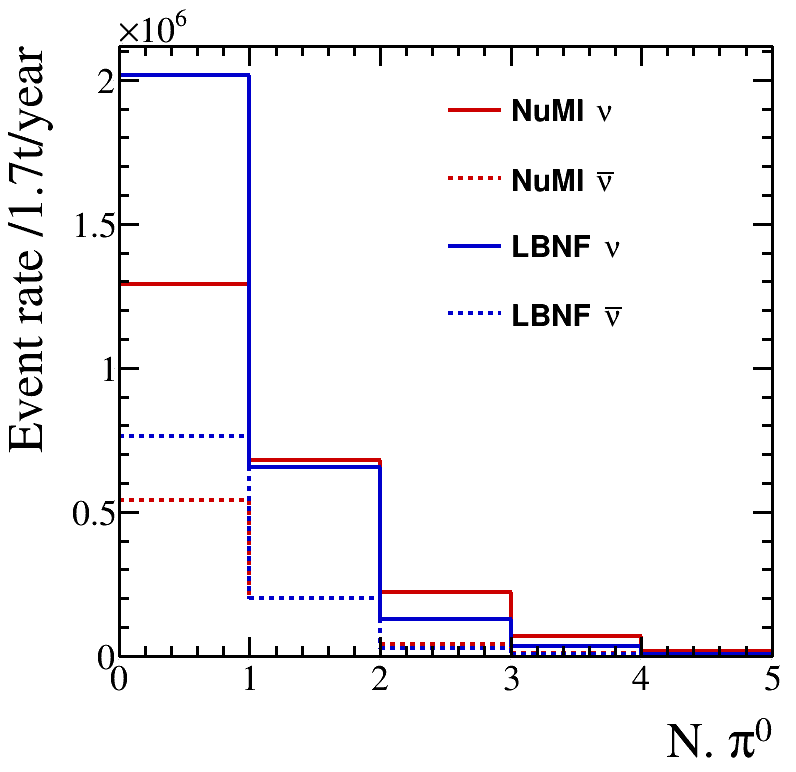
\includegraphics[width=0.5\textwidth]{plots/2x2_npi0_all.png}}
  \subfloat[$\pi^{0}$ kinetic energy] {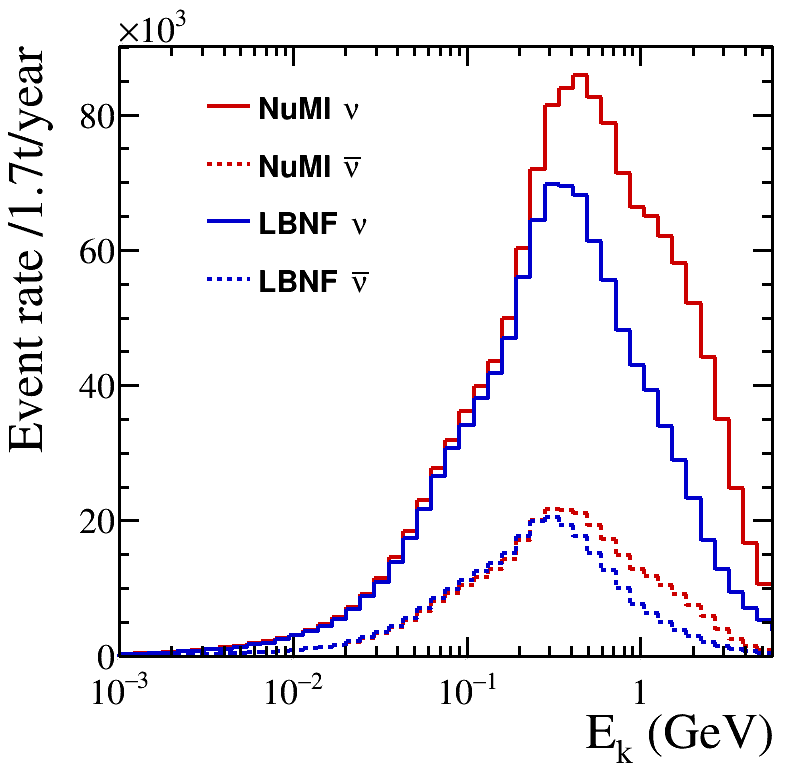
\includegraphics[width=0.5\textwidth]{plots/2x2_pi0_Ek_all.png}}  
  \caption{The expected yearly rates of $\pi^{0}$'s produced at the vertex, as a function of event multiplicity and their kinetic energy, expected in the 2x2 module's 1.7t LAr volume for the NuMI ME and LBNF fluxes, produced using GENIE v2.12.8 with the ``ValenciaQEBergerSehgalCOHRES'' configuration~\cite{genie}. Note that every $\pi^{0}$ from each event is included.}
  \label{fig:pi0_kinematics}
\end{figure}
There are, of course, some qualifiers for this study. Many photon-induced showers will not be contained, and those which are will be lower energy than many EM showers expected in the DUNE ND. Figure~\ref{fig:pi0_kinematics} shows the expected $\pi^{0}$ production rate in the active volume of the 2x2 demonstrator module in the LBNF NuMI ME beamlines, as a function of $\pi^{0}$ multiplicity in each event and $\pi^{0}$ kinetic energy. Two further issues for this study are apparent. Firstly, events with more than one $\pi^{0}$ introduce a problem: even if two EM showers are fully contained, they may not come from the same $\pi^{0}$ decay. Secondly, of those $\pi^{0}$ decays for which both photons are fully contained, the initial $\pi^{0}$ is likely to have a low kinetic energy, which is likely to exclude some fraction of the events. However, despite these challenges, a measure of EM shower resolution from ProtoDUNE-ND would be very useful for DUNE ND design studies, so this possibility is worth investigating further.

\todo{Patrick: add ArgonBox study on this. Need: Event display examples of fully contained pi0 decay events. Efficiency for containing photons as a function of photon energy. Efficiency of containing two photons as a function of pi0 kinetic energy.}
\todo{James, do you have any other comment on photon/electron separation? I decided this would be a better thing to aim for for Patrick's studies}
\FloatBarrier
\subsection{Michel tagging}
\todo{Figure out if we can do anything remotely reasonable... Patrick could see how many stopped muons/pions he has. But I'm not sure how we get the efficiency from that...}

\subsection{Proton tagging}
\todo{Worth commenting on figuring out how well we can find Bragg peaks? Do we care for this test?}

\subsection{Electric field uniformity and space charge build-up}
A concern for LAr detectors in a high intensity beam is the build up of space charge --- long-lived argon ions which drift slowly towards the cathode --- and possible affects on the uniformity of the electric field which may accumulate over time. In currently operating and near-future LAr detectors~\addcite (uB and SBND), both cosmic tracks and UV lasers are used to calibrate for distortions in the electric field. Both the UV laser track and high energy cosmic muons are expected to leave straight tracks in the detector. If the drift field is not uniform across the detector, ionization electrons produced along the length of this track will not drift at the same speed, and will result in a distorted track at the readout plane. By comparing the reconstructed and expected track, a map of the electric field distortion can be built up for calibration purposes.

Assuming that the 2x2 demonstrator module is equipped with scintillator panels to tag cosmic tracks using a timing coincidence between two sides of the detector, and reasonable spatial resolution on those scintillator paddles, electric field distortions could be measured in the 2x2 demonstrator module. By looking at beam-on, and beam-off data, it would be possible to look at the possible affect of space charge build-up over time due to the high event rate in the NuMI beam. If significant space charge build-up were observed, this would inform the future ArgonCube ND design, as a higher drift field strenght would be required. \todo{Is this utter horseshit?}.

Additionally, although the electric-field uniformity of the resistive field shell will be checked in a small scale LAr TPC at Bern, a check of the electric-field uniformity and stability over time for full-size ArgonCube modules would be a valuable final validation of the design.

\subsection{Cosmic suppression}
\todo{James, check whether this word salad makes sense}

The DUNE ND will be a surface detector, with a relatively small overburden. ArgonCube, and all LAr TPCs are slow detectors, with long drift times, over which multiple cosmics will leave tracks in the detector. Although fast timing from the light collection system can, in principle, strongly suppress the cosmic background, this is a reconstruction challenge. A key design choice for the DUNE ND is whether or not a cosmic ray tagging system is required --- for example, a series of scintillator planes surrounding the LAr TPC, as for SBND and MicroBooNE~\addcite. The proposed ProtoDUNE-ND test experiment can help inform this design choice, assuming that the 2x2 Demonstrator module is equipped with scintillator paddles.

By using the scintillator paddles to tag cosmic events using a timing coincidence, methods for rejecting cosmics can be validated independently. For example, we expect that the good timing resolution and light localization from ArcLight will allow cosmics out of the beam window to be rejected with a high efficiency. Additionally, if a cosmic muon traverses a pixel plane, or an ArcLight plane, we would expect to see a large charge deposition or a large number of photoelectrons measured, which could be an additional way to reject cosmic muons. Both of these methods can be validated with ProtoDUNE-ND.

\subsection{Reconstruction with multiple subdetectors}
Because the ArgonCube 2x2 Demonstrator module is relatively small, many events from the NuMI ME beam will not be contained. Figure~\ref{fig:leaky_event} shows a neutral current event where many pions are produced, but in which the pions and subsequent hadronic showers extend far beyond the detector. Such events are likely to be uncontained even in the full \todo{what size???} ArgonCube component of the DUNE ND. In charged-current events, the muon will be uncontained most of the time. For this reason, and because it is not possible to magnetize the large LAr component, a magnetized tracking detector is proposed downstream of ArgonCube in the DUNE ND. A test module for the HPTPC is hoped to be included as part of the ProtoDUNE-ND effort as described in Section~\ref{sec:hptpc-design}. With multiple subdetectors included in ProtoDUNE-ND, multi-detector reconstruction capabilities can be developed and tested. Additionally, if the sign and momentum of escaping hadrons and muons can be measured, it may be possible to make physics measurements with ProtoDUNE-ND, which would be beneficial to the overall DUNE program. For that reason, if no downstream tracker is available, it would be highly desirable to utilize the proximity of the MINERvA and MINOS-ND detectors, and try to minimze the distance between the ArgonCube 2x2 demonstrator and those detectors, in order to use them as downstream trackers.
\begin{figure}[htb]
  \centering
  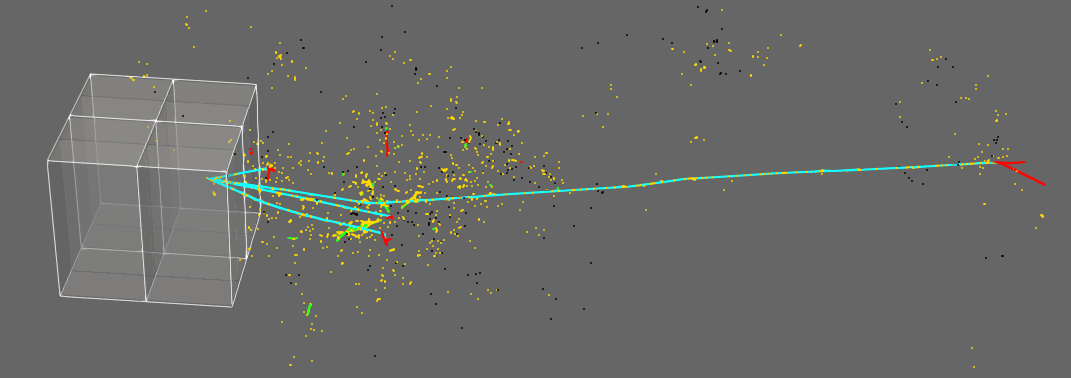
\includegraphics[width=0.8\textwidth]{{plots/EventDisplays/8.17GeV_rectangle_crop}.png}
  \caption{Example ArgonBox simulated event for an 8.17 GeV $\nu_{\mu}$--argon neutral-current multi-pion interaction, in which the pions are not contained in the module. Energy deposits in a bulk volume of LAr are color-coded according to the particle type: $\pi^{\pm}$ --- blue; $\mu^{\pm}$ --- purple; $e^{+}$ --- green; $e^{-}$ --- yellow; proton --- red; recoiling nuclei --- black. The event vertex was randomly placed inside the active volume of the 2x2 demonstrator module, the geometry for which is superimposed on these images, but which is not simulated by ArgonBox.\todo{Can the full size ND be superimposed on this as well?}}
  \label{fig:leaky_event}
\end{figure}
